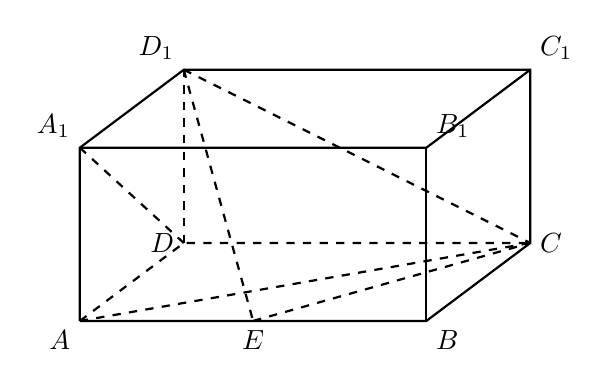
\begin{tikzpicture}[scale=1.1,>=stealth]
  % 顶点坐标
  \coordinate (A) at (0, 0);
  \coordinate (B) at (4.0, 0);
  \coordinate (D) at (1.2, 0.9);
  \coordinate (C) at (5.2, 0.9);

  \coordinate (A1) at (0, 2.0);
  \coordinate (B1) at (4.0, 2.0);
  \coordinate (D1) at (1.2, 2.9);
  \coordinate (C1) at (5.2, 2.9);

  % 点 E 位于 AB 上
  \coordinate (E) at (2.0, 0);

  % 长方体可见棱
  \draw[thick] (A) -- (B) -- (C) -- (C1) -- (D1) -- (A1) -- (A);
  \draw[thick] (A1) -- (B1) -- (C1);
  \draw[thick] (B) -- (B1);

  % 长方体内部不可见棱 (虚线)
  \draw[dashed, thick] (A) -- (D) -- (C);
  \draw[dashed, thick] (D) -- (D1);

  % 辅助线与线段 (虚线)
  \draw[dashed, thick] (D1) -- (E);
  \draw[dashed, thick] (E) -- (C);
  \draw[dashed, thick] (D1) -- (C);
  \draw[dashed, thick] (A) -- (C);
  \draw[dashed, thick] (A1) -- (D);

  % 顶点标签
  \node[below left] at (A) {$A$};
  \node[below right] at (B) {$B$};
  \node[right] at (C) {$C$};
  \node[left] at (D) {$D$};
  \node[above left] at (A1) {$A_1$};
  \node[above right] at (B1) {$B_1$};
  \node[above right] at (C1) {$C_1$};
  \node[above left] at (D1) {$D_1$};
  \node[below] at (E) {$E$};
\end{tikzpicture}
